\section{Planning, validation and reflection}
\label{sec:planning}

\begin{upshot}
\item \textbf{Intent held in state makes progress checkable. Reader judgement becomes a runtime
  predicate.} A plan records what the run is for, and a completion condition attached to a step
  converts progress from a judgement a reader makes into a predicate the runtime evaluates.
\item \textbf{Feedback changes a run at two levels.} An observation that agrees with the plan
  changes the next action alone; an observation that contradicts it changes the remaining plan.
  Rewriting the remaining plan is the event a planner exists for, and counting ordinary progress as
  one makes a planner expensive without making it useful.
\item \textbf{Independent acceptance requires both a separate check and a trustworthy signal.}
  Asking a model to ``check its work'' supplies neither independent control over acceptance nor
  external evidence of correctness. Without an external signal, self-assessment can lower accuracy
  while adding calls. The workflow therefore gives mechanical checks control over acceptance and
  confines the model-based validator to rejection.
\item \textbf{A refused attempt leaves behind guidance, not its context.} Reflection turns a
  refusal into text that outlives the attempt reset, and the reset is what separates a second
  attempt from a longer first one.
\end{upshot}

\subsection{The plan as a field of state}
\label{sec:planning-plan}

Planning sounds like something that belongs at design time, and in the chain it did: the order of
operations was the plan that we wrote. What changes here is that the run writes one for itself
while it is running and then has to operate with what it wrote.

\begin{definition}[Open-loop planning]
\label{def:open-loop}
A planning agent is \emph{open-loop} when the whole plan over the horizon is fixed by the initial 
planning policy and never revised.
\end{definition}

\begin{definition}[Implicit closed-loop planning]
\label{def:implicit-closed-loop}
A planning agent is \emph{implicitly closed-loop} when the plan is held at its 
initial value and feedback modifies a single action: such a system maintains 
$P_t = P_0$ and ``only modify[s] a single action based on the feedback'' \citep[\S2]{sun2023adaplanner}. 
\end{definition}

\begin{definition}[Explicit closed-loop planning]
\label{def:closed-loop}
A planning agent is \emph{explicitly closed-loop} when feedback revises the plan itself, 
following ``the policy $\rho(P_t|g, c_t, P_{t-1})$, where $P_t \in \Delta(A^{T-t})$ is the refined plan 
at time step $t$ containing the modified future actions $a'_{\geq t}$ to execute and $P_{t-1}$ is the 
old plan modified in the previous time step'' \citep[\S2]{sun2023adaplanner}.
\end{definition}

Our reactive loop sits off this axis entirely, it has no plan to hold fixed or to revise. AdaPlanner
files ReAct and Reflexion among the methods whose feedback changes the action rather than the plan,
with no decomposition of the task into subgoals \citep[Table~1]{sun2023adaplanner}. And, to
be honest, that is a fair description of what we built. The context grows with each observation, 
and the next action is chosen from it.

Now, the mechanism that makes an explicit plan worth holding is not the list of subgoals. It is what
AdaPlanner attaches to each one, where ``each subgoal ends with an assertion statement to test its
fulfillment, which allows our method to interact actively with the environment and later resume its
execution with a refined plan'' \citep[\S3.1]{sun2023adaplanner}. \textbf{And, an assertion is a
completion condition written at plan time and evaluated by the runtime, which is exactly the object
the loop was missing.}

An executable assertion separates two questions: who decides what counts as completion, and who
checks whether that condition holds? Here, the planner writes the condition and the runtime
evaluates it. Execution establishes whether the condition holds, not whether it captures the task's
actual requirements. An assertion is therefore still a signal, subject to the fourth claim above:
every subgoal can pass its check while the alert that started the run remains unresolved.
\textbf{The runtime checks the planner's definition of completion; it does not make that definition
correct.} The three checks in \demoref{submit}, by contrast, are conditions we wrote and the runtime
evaluates. That is why \cref{sec:validation-evidence} rests on those checks rather than on the
plan's own assertions.

An explicit plan records subgoals, proposed actions, and completion conditions; it need not be
executable code. For example, a plan can record a structured condition such as
\texttt{status = resolved}, name a predefined check such as ``all required tests pass,'' or
state a prose criterion such as ``the response addresses every item in the request.''
The runtime can compare an observed field with the structured condition or invoke the named check;
the prose criterion instead needs to be translated into a check or judged by a model or a human.
These are all ways to record what counts as completion, but only those tied to an executable
check provide a runtime assertion without further interpretation. None guarantees that the
chosen condition captures the task's actual requirements.

AdaPlanner realizes this general structure as Python code, with comments describing
subgoals and code specifying actions and assertions \citep[\S3.1]{sun2023adaplanner}.
This representation makes both the proposed actions and their completion conditions inspectable,
and lets the runtime evaluate the assertions rather than asking a model to interpret prose conditions.

\begin{foodforthought}
Is the agent you are building open-loop, closed-loop, or somewhere between? Decide it by naming what
your run does with an observation that contradicts what it expected: nothing, one action, or the
rest of the work. Then write down what your plan has to record for that answer to be true, and which
of the three forms above each completion condition takes. Last, write the condition that fires a
revision before you write the node that performs one. A planner that revises whenever anything
surprising arrives is an expensive way to track the observations.
\end{foodforthought}


A reactive loop asks the model to choose the next operation for the task as a whole. Adding a
planner narrows that choice: the model chooses an operation for the current subgoal. The plan also
records three things that the reactive loop does not explicitly track: the subgoals to achieve,
the conditions for completing each step, and which parts of the plan to revise when an observation
contradicts it. Adding a validator lets a model reject a candidate, while the runtime still controls
whether it can be released. Planning, revision, and validation require additional model calls.
\Cref{tab:planning-decisions} summarizes these differences.

\begin{table}[htbp]
  \caption{How a planner and a validator change the reactive loop described in
  \cref{tab:reactive-decisions}. The first row shows how the choice of the next operation changes;
  the remaining rows compare goal tracking, completion checks, revision, acceptance, and cost.}
  \label{tab:planning-decisions}
  \small
  \begin{tabularx}{\linewidth}{Xll}
    \toprule
    Decision & Reactive loop & With a planner and a validator \\
    \midrule
    Who chooses the next operation? & The model, for the whole task & The model, for the current subgoal \\
    \midrule
    Where are subgoals recorded? & No explicit plan & In the plan stored in state \\
    What marks a step as complete? & No explicit completion condition & A condition recorded by the planner \\
    What changes when an observation contradicts expectations? & The context & The context and the remaining plan \\
    Who decides whether to accept a candidate? & The runtime applies fixed checks & The runtime; a model can also reject \\
    What limits model calls? & The call budget & The budget must also cover planning and validation \\
    \bottomrule
  \end{tabularx}
\end{table}

Acceptance is the row where a validator gains least. A validator that can refuse a candidate is a
different thing from a validator that can release one, and \cref{sec:validation-evidence} defends
keeping that difference.

\subsection{Three shapes of planner}
\label{sec:planning-shapes}

A planner is defined less by how it writes a plan than by what it does when the world disagrees with
one. Three arrangements answer that differently, and each answers the same four questions: what the
planner sends, what comes back, what changes when it does, and what the arrangement costs.

\bi

\item \textbf{Open-loop.} The planner sends the whole action sequence at once and nothing comes
back. Nothing changes, because there is no return path along which a change could arrive. One
planning call buys the entire run, which is the cheapest of the three and the only one that cannot
notice that its plan has stopped being right.

\item \textbf{Implicit closed-loop.} The planner sends one action at a time and every observation
comes back to it. What changes is the next action; the remaining actions stand as written, since the
plan is held at the value it had when the run started. The cost is a model call per action, and the
exposure is that an error in the original plan is carried to the end by a run that keeps adapting
around it.

\item \textbf{Explicit closed-loop.} The planner sends one action at a time, every observation comes
back, and the observation is then sorted. One that matches what the plan expected feeds the next
action and leaves the plan alone. One that contradicts it returns to the planner, which rewrites the
remainder of the plan and names the step to resume from. The cost is a model call per action plus
one per rewrite, and the rewrites are bounded by checking at one point per subgoal rather than at
every turn, which holds a run to
``the success status only at $N$ crucial points'' \citep[\S3]{sun2023adaplanner}.

\ei

\textbf{A revision replaces the remainder of the plan rather than adding to it, and that is what
separates revising a plan from accumulating context.} \Cref{fig:closed-loop} draws the difference
literally: in the third arrangement the actions from the current step to the end are struck out and
a new tail is written in their place.

Our reactive loop accumulates. Every observation makes the context longer and nothing in it is ever
withdrawn, so a conclusion the run reached at its second turn is still sitting in the transcript at
its twelfth, arguing its case. On this axis the loop sits closest to the implicit arrangement with
the plan removed: feedback changes the next action, and there is no remainder to revise.

\begin{figure}[htbp]
  \centering
  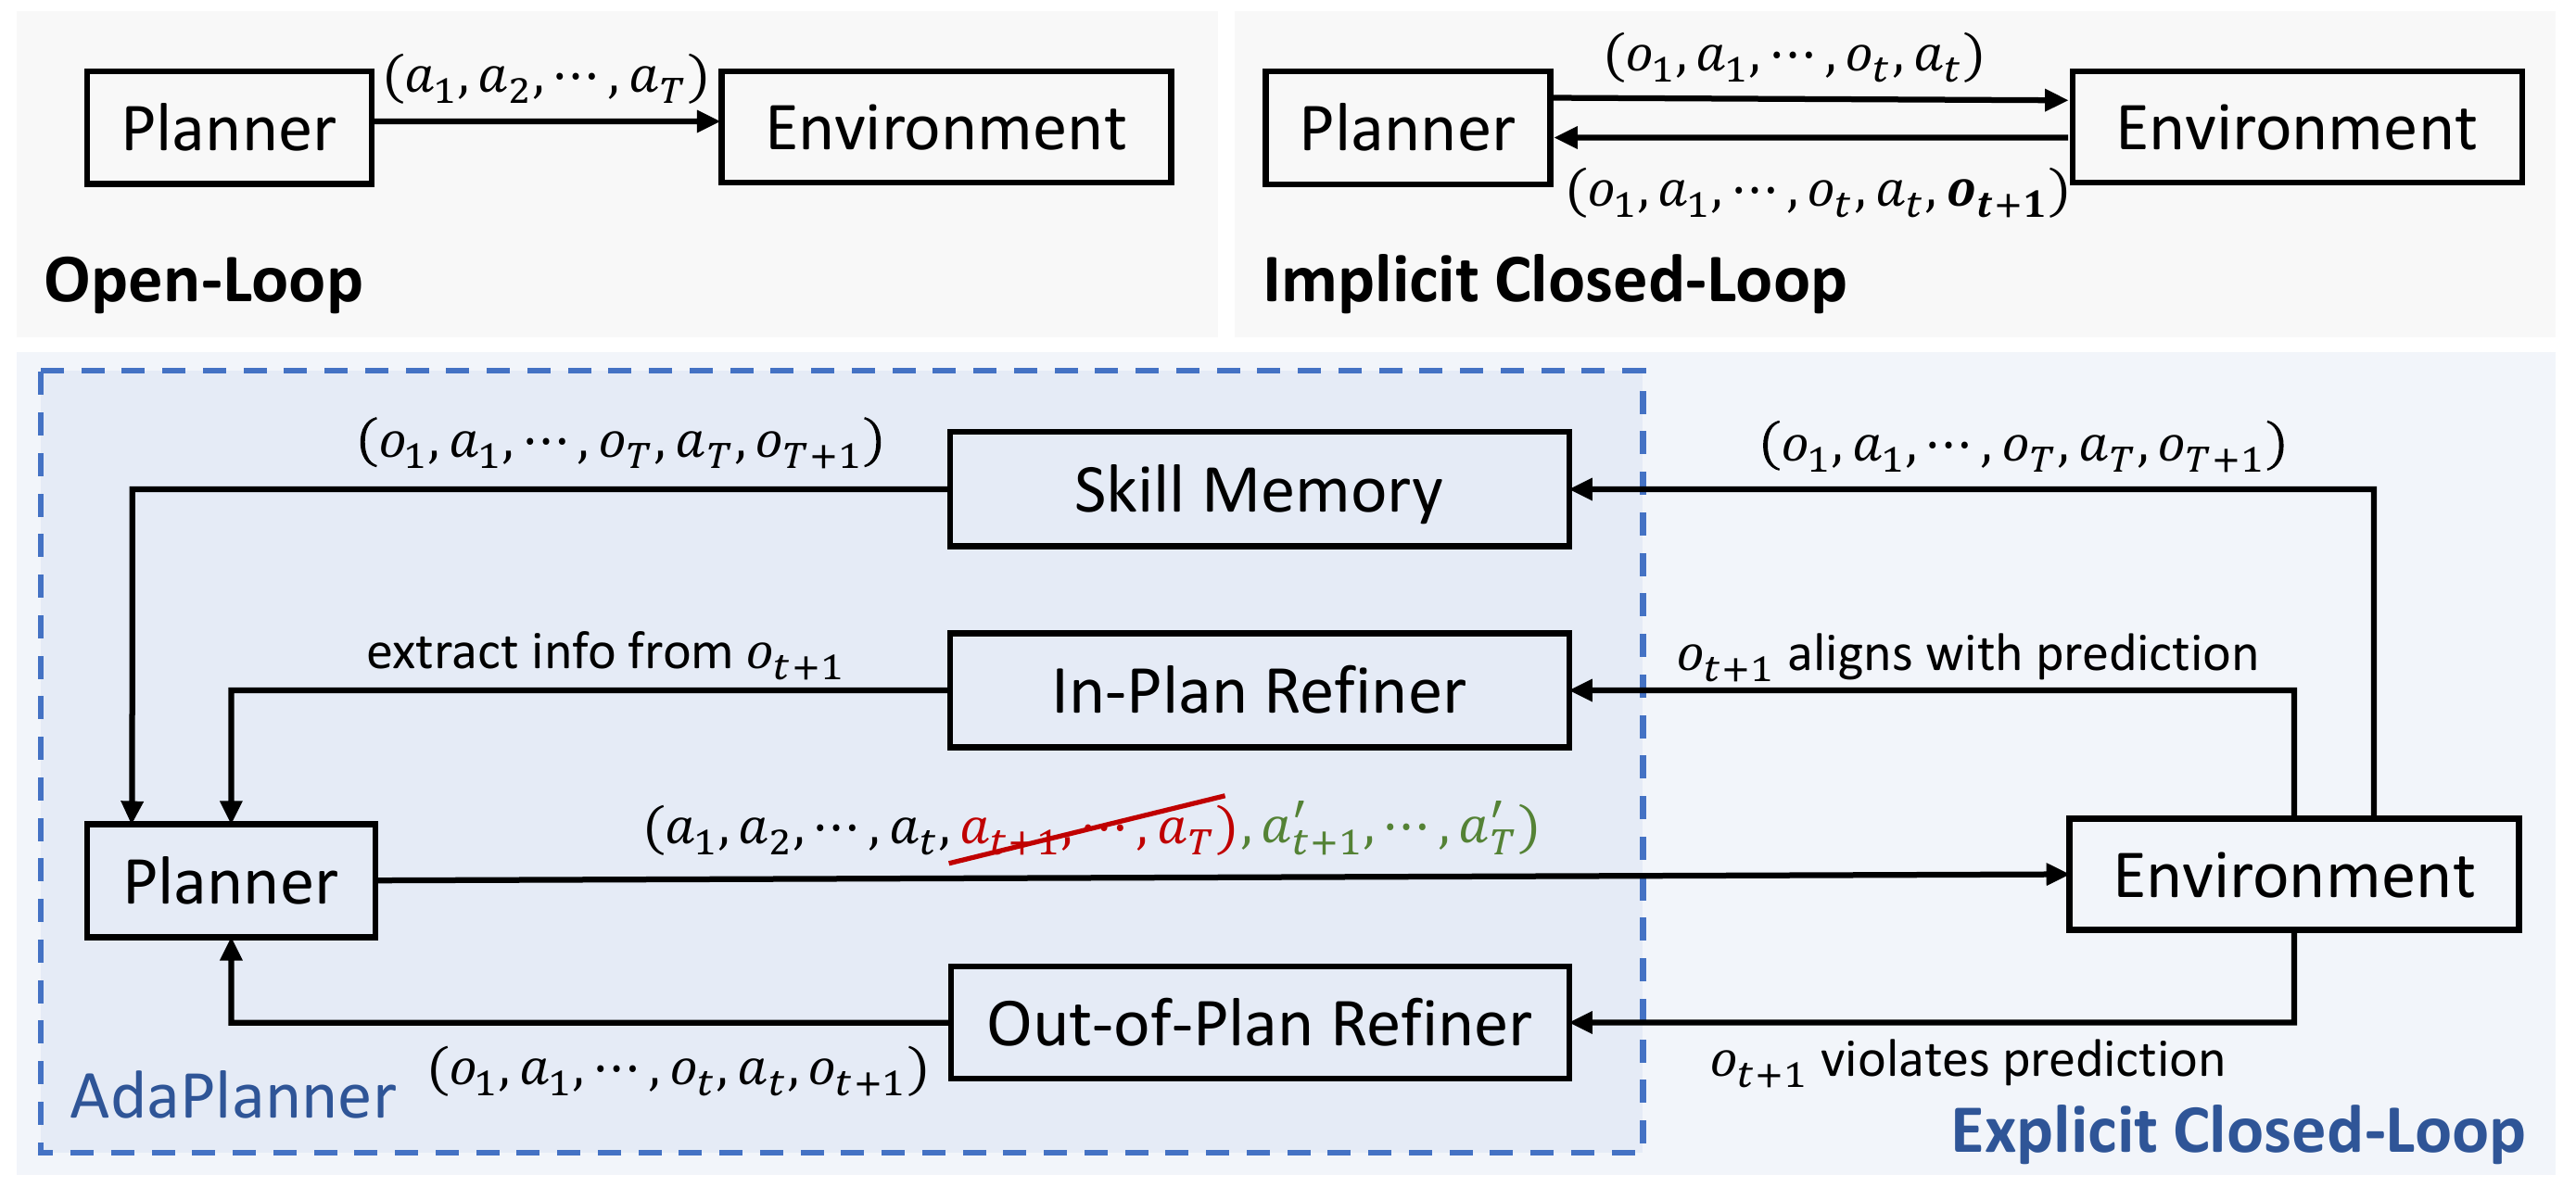
\includegraphics[width=\linewidth]{figures/adaplanner-fig1-closed-loop.png}
  \caption{Open-loop, implicit closed-loop, and explicit closed-loop planning. The left arrangement
  sends actions and receives nothing. The middle one returns each new observation $o_{t+1}$ to the
  planner but holds the plan at $P_0$. The right one sorts $o_{t+1}$ by whether it aligns with the
  prediction or violates it, routes it to the in-plan or the out-of-plan refiner accordingly, and in
  the second case strikes out the remaining actions $a_{t+1},\ldots,a_T$ and writes
  $a'_{t+1},\ldots,a'_T$ in their place. Feedback reaches the planner in both closed-loop
  arrangements; what the explicit one does with it is revise the plan rather than one action, which
  is the difference \cref{def:closed-loop} turns on. Figure~1 of \citet{sun2023adaplanner},
  reproduced for teaching with credit (arXiv non-exclusive licence).}
  \label{fig:closed-loop}
\end{figure}

The sorting step is where the assertion of \cref{sec:planning-plan} does a second job. An
observation can be filed as agreeing or contradicting only where an expectation was recorded before
it arrived, and AdaPlanner ``can anticipate environmental observations and proactively refine the
plan only when there is a discrepancy between expected and actual outcomes''
\citep[\S3]{sun2023adaplanner}. A completion condition closes a subgoal, and it also decides which
return path an observation takes.

The skill memory in \cref{fig:closed-loop} is the one component we do not carry over. It stores plans that
succeeded and offers them back when a later task resembles an earlier one
\citep[\S3.3]{sun2023adaplanner}: memory that crosses from task to task. What
\cref{sec:reflection} needs crosses from attempt to attempt inside one task. The boundary is
different, so we build an attempt memory rather than borrow the skill memory.

\subsection{Revising plans}
\label{sec:planning-revision}

Not every unexpected observation calls for a new plan. Rewriting the plan after every surprise
costs a model call each time and turns it into a record of events rather than a guide to action.
Before implementing a response, we therefore need to distinguish four cases. Only one revises
the plan within the current run.

\bi

\item \textbf{In-plan.} The observation agrees with what the plan anticipated, and what the run
takes from it is information the next action needs. AdaPlanner does this with a dedicated action
that queries the model to parse the observation, so the extracted value flows into later actions
\citep[\S3.2]{sun2023adaplanner}. The plan itself is untouched. This is the loop of
\cref{sec:reactive} with somewhere to put what it learned.

\item \textbf{Out-of-plan.} A subgoal's assertion fails, and the planner regenerates the remaining
plan from the current state. AdaPlanner assembles an error message reporting where the agent is,
what it holds, and its last three interactions, then refines the plan and sets the step to resume
from, so the episode continues from an intermediate point rather than restarting
\citep[\S3.2]{sun2023adaplanner}. This is the one that changes what the run intends to do, and the
mechanism a planner is built around.

\item \textbf{Neither.} On a fixture as small as ours this is the common case. When the model
follows a value into a helper file and finds what it needed, no assertion has failed and the plan
has not been revised: a subgoal has been completed, in the ordinary way, by the step the plan said
would complete it. \textbf{Ordinary progress is not replanning, and counting it as such makes a
planner look busy while it is doing nothing.}

\item \textbf{Not in this run.} A whole attempt is refused, and a fresh plan is written with what
the failed attempt taught. That event ends the run rather than redirecting it, so it belongs to
\cref{sec:reflection}, along with the memory that has to survive the reset.

\ei


\subsection{Does planning make a difference?}
\label{sec:planning-evidence}

Planning is something that is easy to buy into but hard to measure, 
because a system that plans usually differs from a system that does 
not in more ways than the planning.

The question to answer is: does planning improve performance when everything else is held fixed? 
Recent work by \citet{wang2026reasoningplan} tests this question directly. The researchers compare
four ways of choosing the next action: one step at a time, beam search, lookahead, and lookahead
with value propagation, keeping the rest of the agent setup the same.

\textbf{Planning helps, and the gain is not reserved for large models.} The smallest model tested,
planning ahead, outscores a frontier model that chooses one step at a time.

\begin{itemize}
% \item They repeat the comparison in two agent frameworks using four language models
% \citep[\S5.1]{wang2026reasoningplan}.
\item On one benchmark, the smallest model tested, with 8 billion parameters, scores 73.8\% when it chooses
one step at a time. Its score rises to 85.6\% when it looks several steps ahead and uses estimates
of future outcomes to choose its next action, a method called lookahead with value propagation.
\item That is higher than the 78.3\% scored by a frontier model (at that time) choosing one step at a time
\citep[Table~1]{wang2026reasoningplan}.
\end{itemize}

The four rows of \cref{tab:planning-failure} differ only in what an action is scored against.
Choosing one step at a time scores the action itself, and beam search keeps more candidates while
scoring them the same way, so it is wider rather than different in kind. Lookahead scores an action
by simulating the trajectories it leads to and reading off those outcomes instead.

Value propagation is what the fourth row adds. Each simulated outcome is pushed back onto every
action along the way, so an action's value aggregates the futures that run through it, and evidence
from late in a simulation can revise a choice made early. Lookahead without that feedback is not
enough on its own: ``Lookahead alone is insufficient unless information from simulated futures can
revise early decisions'' \citep[\S4.2]{wang2026reasoningplan}.

\Cref{tab:planning-failure} is a more illustrative view because it measures the failure rather than
the success.

\begin{table}[htbp]
  \caption{How four ways of choosing the next action fail, aggregated over three benchmarks. The
  last row is the paper's \textsc{Flare}. Lower is better in the first column, higher in the other
  two \citep[Table~3]{wang2026reasoningplan}.}
  \label{tab:planning-failure}
  \small
  \begin{tabularx}{\linewidth}{Xlll}
    \toprule
    How the next action is chosen & Dead end on move one & Step of first error & Recovers after it \\
    \midrule
    One step at a time & 55.6\% & 1.6 & 5.4\% \\
    Beam search & 71.9\% & 2.0 & 11.4\% \\
    Lookahead & 23.6\% & 2.8 & 22.4\% \\
    Lookahead with value propagation & 17.8\% & 3.2 & 29.7\% \\
    \bottomrule
  \end{tabularx}
\end{table}

Read the top row against \cref{sec:reactive-react}. A run that chooses one step at a time walks into
a branch it cannot come back from on its very first move more than half the time, makes its first
error before the second step, and escapes that error once in twenty. That is the loop which repeats
itself without going anywhere, and these three numbers say what the trajectory could not: the error
arrives almost immediately, and the run then cannot get out.

\textbf{What makes a plan good is what follows from it, and neither more search nor a more
human-sounding plan is the same thing.} The remaining rows, and the two studies after them, are
three ways of finding that out.

Now read the beam-search row, which is the surprise. Beam search searches more than choosing one
step at a time, and it walks into the first-move trap more often. More search over the same
local score does not help, because the score is the problem. What moves the numbers is evaluating an
action by what follows it.

Two results say the representation is part of the mechanism. Stripping only the code interface from
a planner and writing the same plans in language costs it 81\% against 46\%
\citep[Figure~4c]{sun2023adaplanner}. Independently, web agents given plans in a structured formal
representation beat the same agents given free-form plans at i) subgoal completion, 70.3\% against
63.2\%, ii) plan completion, 37.5\% against 34.6\%, and iii) task success, 36.4\% against 32.1\%
\citep[Figure~3]{aghzal2026webagents}. One round of revision after exploring the environment then
carries structured-plan subgoal completion from 70.3\% to 93.3\%.

One finding in that study separates a good plan from a plan that looks right. Revision moves the
agent's plan \emph{away} from the human-written plan while improving what the agent achieves, with
exact matches against the human plan falling from 67.7\% to 59.0\%
\citep[Table~2]{aghzal2026webagents}. Resemblance to the plan a person would have written moves in
the opposite direction to the thing we are trying to improve.

Four things bound all of this.

\bi

\item \textbf{Task.} Neither study is program repair. One is knowledge-graph question answering, the
other is live web navigation.

\item \textbf{Environment.} The failure numbers come from ``oracle-structured subgraphs that
guarantee the existence of valid solution paths'' \citep[\S5.1]{wang2026reasoningplan}, so the
environment is deterministic, fully observable, and known to be solvable. Ours is none of the three,
and for some alerts no patch exists at all.

\item \textbf{Mechanism.} Simulating candidate futures and scoring them is not what our planner
does. What it shares with writing subgoals and completion conditions is only that early decisions
are made to answer to later evidence, so it validates the family and not the member.

\item \textbf{Judge.} The web-agent task success rate tops out at 45.1\%, its errors sit mostly
below the plan rather than in it, and it is scored by a model judge of the kind
\cref{sec:validation-evidence} spends its length warning about
\citep[\S4.2, \S5.2]{aghzal2026webagents}.

\ei

What survives those bounds is the shape rather than any rate. A run whose early actions answer only
to local scores commits early and cannot recover, and giving those actions something later to answer
to is what changes the outcome.

\subsection{The proposer and the judge}
\label{sec:validation}
\label{sec:validation-actor}

Acceptance has been the runtime's job since the chain, and nothing so far has asked whether the
runtime is any good at it. The three checks in \demoref{submit} are cheap and they are dull, and
both of those turn out to be load-bearing properties rather than shortcomings.

\begin{definition}[Actor and evaluator]
\label{def:actor-evaluator}
An agent separates \emph{proposal} from \emph{assessment} when the component that produces a candidate is not the component that scores it. Reflexion draws the split as two of three models: ``an Actor, denoted as $M_a$, which generates text and actions; an Evaluator model, represented by $M_e$, that scores the outputs produced by $M_a$'' \citep[\S3]{shinn2023reflexion}. The evaluator ``takes as input a generated trajectory and computes a reward score that reflects its performance within the given task context'', and it may be an exact-match grader, a heuristic written for the task, or another instance of a language model \citep[\S3]{shinn2023reflexion}.
\end{definition}

Self-Refine draws the same picture with one model in all three roles. It generates an output,
prompts the same model for feedback on that output, and prompts it again to revise, with three
prompts and no training \citep[\S2]{madaan2023selfrefine}. What matters for us is where its loop
exits, because the stopping condition ``either stops at a specified timestep $t$, or extracts a
stopping indicator (e.g.\ a scalar stop score) from the feedback''
\citep[\S2]{madaan2023selfrefine}, and the feedback is written by the model whose work is being
assessed.

Our loop exits on a value the runtime wrote. That difference does not show up in a diagram of boxes
and arrows, and it is not something a prompt can establish. \textbf{The accepting decision belongs
to whichever component writes the value the exit edge reads, which is a fact about the graph we
compiled and not about anything we asked the model to do.} Instruct a model to be strict with itself
and it remains the author of the number the edge tests.

So the question in front of us is not whether to separate the proposer from the judge, because
\demoref{submit} has been separate from the controller since the chain. The question is what a
second model adds to a separation we already have, and what it costs to let that model hold the
decision.

\subsection{What a model judge can and cannot see}
\label{sec:validation-judge}

Each check answers its question with a program rather than an opinion: i) the patch applies, so the
edit is well formed; ii) it touches the flagged line, so the run addressed its alert; iii) the
rescan is clean, so the scanner is quiet. Each is fast, each is reproducible,
and none of them needs a model.

Here, a verifier is \emph{sound} when it never accepts an incorrect solution, and \emph{complete}
when it never refuses a correct one. Soundness on its own buys nothing, because a verifier that
refuses everything never accepts an incorrect solution. \textbf{Completeness is what carries the
property the argument below rests on: a verifier that produces no false refusals leaves a system no
worse off than not checking at all, because anything generated correctly is still accepted.} The
external verifiers behind the gains in \cref{sec:validation-evidence} are both at once, being
decision procedures for their domains.

Our three checks are neither. A scanner that reports nothing has not established that nothing is
there, and an edit that renames the flagged expression or moves it behind a wrapper can clear an
alert while leaving the weakness in place, which is a false acceptance. A correct patch that fixes
the weakness somewhere other than the flagged line fails the second check, which is a false refusal.
What the checks are is cheap and reproducible, and the error to avoid is reading them as though they
were sound.

That gap is the validator's job, and it is a narrow one. Given the alert, the candidate patch, the
results of the three checks, and the trajectory that produced them, a validator can ask three
questions the checks cannot.

\bi

\item \textbf{Weakness or alert.} Does the patch remove the unsafe behavior, or does it remove the
scanner's ability to see it? This is the validation-retreat failure of \cref{sec:reactive-react}
under a different name, and on this fixture it is the failure most worth catching.

\item \textbf{Behavior.} Does the edit change what the endpoint returns? The performance measure
cares and none of the three checks looks.

\item \textbf{Provenance.} Did the run actually establish what its patch assumes, or did it assert
it? The trajectory is in front of the validator and was never in front of the checks.

\ei

\subsection{Why the judge does not decide acceptance}
\label{sec:validation-evidence}

Having found something for a second model to do, we now have to decide how much authority it gets,
and the evidence on that question is unusually one-sided.

Start with the setting the results are about. \emph{Intrinsic} self-correction is the case in which
a model revises ``based solely on its inherent capabilities, without the crutch of external
feedback'' \citep[\S1]{huang2024selfcorrect}, which is precisely the case where a validator holds
the accepting decision and nothing else does. Measured that way on reasoning benchmarks, accuracy
falls while cost rises: one model answers a grade-school mathematics benchmark at 95.5\% in a single
call, 91.5\% after one round of self-correction across three calls, and 89.0\% after two rounds
across five \citep[Table~3]{huang2024selfcorrect}. The same pattern appears on a commonsense
benchmark, where a weaker model falls from 75.8\% to 38.1\% after one round
\citep[Table~3]{huang2024selfcorrect}.

Supply the ground-truth label instead, so that correct answers are never revised, and the same
procedure improves that mathematics result from 95.5\% to 97.5\%
\citep[Table~2]{huang2024selfcorrect}. The gain is real and it is not available: ``If we are already
in possession of the ground truth, there seems to be little reason to deploy LLMs for
problem-solving'' \citep[\S3]{huang2024selfcorrect}. Two systems whose reported improvements rest on
that setup are named, and one of them is Reflexion \citep[Table~1]{huang2024selfcorrect}, which
matters for how we read \cref{sec:reflection}.

A second study separates the verifier from the generator and varies only the verifier. Across 100
instances per domain with one model, self-critique moves a graph-coloring result from 16\% to 2\%
and a Game of 24 result from 5\% to 3\%. Replacing the model verifier with a sound one moves the
same two results to 38\% and 36\% \citep[Table~1]{stechly2025selfverification}. On a
blocks-planning domain self-critique does help, from 40\% to 55\%, and a sound verifier still beats
it at 60\% to 87\% depending on how much detail the critique carries
\citep[Table~1]{stechly2025selfverification}.

The verifier's error profile explains the collapse. Used as a verifier, the model reaches 72.4\%
accuracy on graph coloring, refusing 95.8\% of the correct answers it saw and accepting 6.5\% of the
incorrect ones, and 79.6\% on a disguised blocks domain, where those two rates are 97.09\% and 0.5\%
\citep[Table~2]{stechly2025selfverification}. A judge
that refuses nearly every correct answer does not merely fail to help, because ``the system rejects
most answers and then times out on a set of later, worse generations''
\citep[\S5]{stechly2025selfverification}. The acceptance error runs the other way. On the two
domains where the judge does least badly it accepts 10.4\% of incorrect Game of 24 answers and
18.55\% of incorrect blocks plans, against 6.5\% and 0.5\% on the two where it refuses almost
everything \citep[Table~2]{stechly2025selfverification}.

One finding sets our design rule. Once the verifier is sound, binary feedback, feedback naming the
first error, and feedback naming every error land within four points of one another on three of the
four domains. Those readings are 38\%, 37\% and 34\% on graph coloring, 36\% against 38\% on Game of
24, and 10\%, 8\% and 6\% on the disguised blocks domain. On blocks planning they do not, running 60\%, 87\% and
83\%, so there naming the first error is worth twenty-seven points over a bare refusal
\citep[Table~1]{stechly2025selfverification}. \textbf{What a loop needs first from its judge is a
trustworthy accept-or-reject bit; what an attached explanation adds on top of that ran from nothing
to twenty-seven points across the four domains.} Dropping the critique altogether and sampling
repeatedly does at least as well on two of them, reaching 44\% on graph coloring and 42\% on Game of
24 at twenty-five samples \citep[Table~1]{stechly2025selfverification}.

These are four reasoning and planning domains with one model family, not program repair, and repair
has something those domains lack: a rescan and a test suite are real programs that run. What
transfers is the error profile of the source rather than a rate we can borrow. Where the accepting
signal comes from a model, the outcome follows that model's error rates rather than the idea. The
loop collapses on the two domains whose false-refusal rates run above 95\%, and on blocks planning, where that rate is
15.48\%, it gains fifteen points where a decision procedure gains twenty to forty-seven
\citep[Tables~1 and 2]{stechly2025selfverification}. Where the signal comes from a verifier that is
correct in both directions, the loop improves on all four. Our three checks are programs and they
are correct in neither direction, so what they inherit is reproducibility rather than the
guarantee.

That is why the mechanical checks keep the accepting decision. \textbf{The validator may refuse a candidate that
passed all three checks, and it may not release one that failed them.} Confined that way, the only
error it can make is refusing work that was already finished, and a refusal costs a turn against a
budget we set. Were it allowed to release, its false acceptances would end the run, and nothing
downstream would look again. Given false-negative rates of the size measured above, a judge confined
to refusal can still stall a run by refusing everything, which is what the attempt cap of
\cref{sec:reflection} is for.

\Cref{sec:fixed} and \cref{sec:reactive} both promised that acceptance would move to something that
did not write the patch, and it has. \demoref{submit} is that something, and the validator is a
second one standing beside it. Neither section promised that the judge would be a model, and the
evidence above is why we do not make it one.

\subsection{What survives a refusal}
\label{sec:reflection}

A refusal ends an attempt, and it need not end everything the attempt learned. What crosses that
boundary is a design decision, and the two obvious answers are both wrong.

The loop itself is short. The validator refuses a candidate, the attempt limit permits another try,
and the runtime starts the next attempt from a cleared record. Something has to change between the
two, or the second attempt is the first one repeated at twice the price. What changes is the
context the next attempt begins with, and we get to choose what goes into it.

\bi

\item \textbf{The whole trajectory.} Too large to carry, and it is the accumulation we were trying
to get out of. An attempt that inherits every observation of the attempt before it is a longer first
attempt wearing a new label.

\item \textbf{The patch.} The artifact that just failed. Carrying it invites the next attempt to
defend it, which is the one thing we do not want a fresh attempt doing.

\item \textbf{The thought.} The action that changes the context and touches nothing else
(\cref{sec:reactive-loop}). It costs a model call, it has no effect in the environment, and it is
the only one of the three that is smaller than what produced it.

\ei

\begin{definition}[Reflection step]
\label{def:reflection}
A reflection step converts the outcome of a failed attempt into text that conditions later attempts.
Reflexion adds it as the third of its three models, ``a Self-Reflection model, denoted as $M_{sr}$,
which generates verbal reinforcement cues to assist the Actor in
self-improvement'' \citep[\S3]{shinn2023reflexion}. Given ``a sparse reward signal, such as a binary
success status (success/fail), the current trajectory, and its persistent memory'', it produces
feedback that ``is then stored in the agent's memory'' \citep[\S3]{shinn2023reflexion}.
\end{definition}

Two lifetimes come with that arrangement, and they are the same two our state record keeps: ``the
trajectory history serves as the short-term memory while outputs from the Self-Reflection model are
stored in long-term memory'' \citep[\S3]{shinn2023reflexion}. The trajectory dies with the attempt;
the reflection does not.

Our reflection node runs on rejection and writes one short entry from four inputs: the alert, the
candidate patch, the validator's reasons, and the trajectory that produced them. The entry appends
to \demoref{reflections}, which survives the reset, while the observations, the plan, the candidate
and the validation are cleared for the new attempt. The counters survive too, so the budget of forty
model calls still binds across both attempts rather than restarting with each one.
\textbf{The reset is what makes the guidance worth anything, because guidance delivered alongside
the context that produced the failure is just more context.} Which fields are cleared, and why
clearing an appending field takes an explicit assignment, is the state machinery of Part~B.

What this does not buy is a second opinion from nowhere. The signal our reflection step receives is
the validator's rejection reasons, which are the three mechanical checks plus a model's objections,
and \cref{sec:validation-judge} said what those checks are worth: they are neither sound nor
complete. The measurements in \cref{sec:validation-evidence} were about revision with no external
signal at all, and this is not that case, but it is not the ground-truth case either. What we expect
is improvement where the failure was legible in the reasons the run was given, and no improvement at
all on an alert for which no patch exists. The attempt cap is there because neither outcome
announces itself.

\subsection{What we gain and what we lose}
\label{sec:planning-tradeoff}
\label{sec:validation-tradeoff}

The planner, the validator and the reflection step are additions of one kind: none of them takes a
decision away from us. We wrote the plan schema, the assertion format, the validator's authority,
the routing predicates and the reset contract, and every one of those is still design time. What we
hand over is a second and a third kind of content decision, and each arrives with its own kind of
error.

\subsubsection{What we gain}

\bi

\item \textbf{Measure.} Progress becomes a predicate. A turn can fall short of a condition the run
itself wrote down, which is the thing \cref{sec:reactive-tradeoff} said no rule over observations
could supply.

\item \textbf{Intent.} The plan is a readable field of state, so a person watching a run can see
what it believes it is doing before it finishes doing it. The trajectory of \cref{sec:reactive-demo}
held four thoughts and nothing a reader could hold the run to.

\item \textbf{Address.} A failure recovers part of the address that \cref{sec:fixed-tradeoff} gave
us and \cref{sec:reactive-tradeoff} spent: the subgoal whose condition failed names where the run
stopped making progress, even though it does not name why.

\item \textbf{Refusal.} A patch that passes all three mechanical checks can still be turned back,
which closes the one gap those checks were always going to leave open.

\item \textbf{Memory.} A refused attempt leaves guidance behind, so a second attempt starts from
what the first one was told rather than from the empty context the first one started in.

\ei

\subsubsection{What we lose}

\bi

\item \textbf{Calls.} Planning costs a call and every revision costs another. Against a fixed budget
these compete with the executor's calls, so a run that replans twice has fewer turns left to act.

\item \textbf{Commitment.} A plan the model wrote badly is now something the run is committed to,
and a bad plan is more durable than a bad turn. The loop could abandon a bad idea by having a
better one; a planner has to detect that the plan is wrong before it can replace it.

\item \textbf{Judgement.} A second model is a second source of error, and its refusals are
expensive in a way its silence is not. A validator that refuses good work spends the budget on work
that was already done.

\item \textbf{Attempts.} The attempt loop multiplies everything beneath it, because a second attempt
pays for a second plan, a second set of turns and a second validation against the same budget. The
guidance it starts from was written by the model whose attempt failed.

\ei

Of what \cref{sec:fixed-tradeoff} called shape, address and termination, these three additions
return neither shape nor termination, and they return the address only as far as the failed
subgoal. We still cannot cost a run before it starts, the attempt cap replaces termination with a
counter we set, and the accepting decision stays with the three mechanical checks, because neither
the validator nor the reflection step is safe to hold it.

\subsection{The demo: the planner and the validator}
\label{sec:planning-demo}
\label{sec:validation-demo}

Both additions are one program, \demoref{demo/lec2\_planning\_and\_validation\_agent}, sitting
beside these notes. One alert runs it:

\begin{lstlisting}[basicstyle=\ttfamily\scriptsize, frame=none]
python -m lec2_planning_and_validation_agent --alert-id bc284c6b
\end{lstlisting}

\noindent Its own README says why the two arrive together: the package holds two segments in one
graph, both are always compiled, and so one run shows both. \Cref{fig:graph-plan-validate} is that
graph, with every node named by the code that implements it.

\begin{figure}[htbp]
  \centering
  \resizebox{\linewidth}{!}{% The DAG of lec2_planning_and_validation_agent, with each component named by the
% code that implements it. Line numbers are that package's graph.py.
\begin{tikzpicture}[x=1cm, y=1cm,
  st/.style={gnode, align=center, minimum width=2.9cm, minimum height=1.3cm, inner sep=3pt},
  mst/.style={st, fill=ibmblue!12},
  rst/.style={st, fill=black!6},
  fl/.style={-{Stealth[length=2.4mm]}, thick, draw=ibmfg!85},
  bk/.style={fl, dashed},
  ev/.style={font=\sffamily\footnotesize, align=center, fill=white, inner sep=2.5pt},
  pred/.style={font=\ttfamily\scriptsize, text=ibmblue!75!black, align=center, fill=white, inner sep=2pt}]
  \def\cond#1{\\[-1pt]{\footnotesize\color{ibmfg!70}#1}}
  \def\code#1{\\[0pt]{\ttfamily\scriptsize\color{ibmfg!60}#1}}

  \node[circle, fill=ibmfg, inner sep=2.4pt] (start) at (-7.4,0) {};
  \node[font=\sffamily\footnotesize\bfseries, above=3pt of start] {Start};
  \node[mst] (plan) at (-4.6,0)    {\textbf{plan}\cond{writes the plan}\code{plan() 182--226}};
  \node[mst] (ctrl) at (0,0)       {\textbf{controller}\cond{one model call}\code{controller() 249--267}};
  \node[rst] (tools) at (0,-4.0)   {\textbf{tools}\cond{execute, observe}\code{tools() 287--322}};
  \node[rst] (sub)  at (5.4,0)     {\textbf{submit}\cond{three checks}\code{submit() 323--354}};
  \node[mst] (val)  at (5.4,-4.0)  {\textbf{validate}\cond{the judge}\code{validate() 355--385}};
  \node[circle, draw=ibmfg, thick, inner sep=3.2pt] (end) at (5.4,-6.4)
        {\tikz\node[circle, fill=ibmfg, inner sep=2.2pt]{};};
  \node[font=\sffamily\footnotesize\bfseries, below=3pt of end] {End};

  \draw[fl] (start) -- (plan);
  \draw[bk] (plan) -- node[ev, auto]{the plan} (ctrl);
  \draw[bk] (ctrl) -- node[ev, auto, pos=0.26]{tool call\cond{by the model}} (tools);
  \draw[bk] (tools.east) to[bend right=32] node[ev, auto, swap, pos=0.3]{observation} (ctrl.south east);
  \draw[bk] (tools.west) to[bend right=32]
        node[ev, auto, swap, pos=0.62]{nothing new came back\cond{by the runtime}} (plan.south);
  \draw[bk] (ctrl) -- node[ev, auto]{no tool call\cond{by the model}} (sub);
  \draw[bk] (sub) -- node[ev, auto, swap]{checks passed\cond{by the runtime}} (val);
  \draw[bk] (sub.north west) to[bend right=22]
        node[ev, auto, swap]{checks failed} (ctrl.north east);
  \draw[fl] (val) -- node[ev, auto]{accepted} (end);

\end{tikzpicture}
}
  \caption{The DAG of the planning and validation demo, each node labelled with its method and line
  range in \demoref{graph.py}. Blue nodes are the three places where a model decides. The four
  routing predicates are \demoref{after\_plan} (414--417), \demoref{after\_controller} (404--413),
  \demoref{after\_tools} (418--432) and \demoref{after\_submit} (433--438). Compare
  \cref{fig:reactive-loop}: only \demoref{validate} reaches the exit.}
  \label{fig:graph-plan-validate}
\end{figure}

Against the loop of \cref{sec:reactive-demo} exactly two edges changed, and each carries one of
this section's arguments.

\bi

\item \textbf{The edge from \demoref{tools} acquired a second destination.} In the loop it ran
unconditionally back to the controller, and its own comment there called it the line that makes the
agent reactive. Here \demoref{after\_tools} chooses, and the second choice is the planner: when the
recent observations have said nothing new, the runtime replaces the plan instead of ending the run.
The loop ended such a run with \demoref{no\_progress}.

\item \textbf{\demoref{submit} can no longer accept.} It runs the same three mechanical checks and
then routes on the outcome, and only \demoref{validate} reaches \demoref{END} with the run accepted.
That the proposer is not the accepter is therefore a property of the compiled graph, and no prompt
is asked to arrange it.

\ei

The plan itself is an ordinary field of state. The planner writes a list of steps, each with an
\demoref{id}, a \demoref{goal} and the \demoref{evidence} that would settle it, beside a
\demoref{revised} flag that records whether this plan replaced an earlier one. One detail of the
implementation is worth reading, because only a running program produces it. \demoref{observations}
accumulates and cannot be cleared, so immediately after a revision the last three observations are
still the identical ones that triggered it, and both guards would fire again on the next turn. The
run would replan and then die on the turn it recovered. The fix is a high-water mark,
\demoref{replanned\_at}, and both checks read \demoref{observations[replanned\_at:]}.

\paragraph{Two runs.} The recorded runs under \demoref{demo/runs/} are a pair worth reading against
each other. In \demoref{v23-bc284c6b} the executor works for four turns, \demoref{submit} passes all
three checks, and the validator accepts: twenty-five events, and the accepting decision is logged
against the validator rather than the controller. In \demoref{v23-28e37a00} the mechanical checks
fail twice, the run is routed back to the controller both times, and it ends in \demoref{error}
after fifty-two events without the validator ever being consulted. That ordering is the design rule
of \cref{sec:validation-evidence} visible in a trace: the cheap check runs first, and the judge is
never asked about work that has already failed mechanically.

Neither recorded run replans. The edge exists in the compiled graph and no run under
\demoref{demo/runs/} has taken it, so nothing here shows what a revision costs in practice.

\begin{demostub}
Three artifacts are still missing. For in-run revision: a run in which \demoref{after\_tools} routes
to the planner, with the original plan, the observations that said nothing new, and the revised plan
beside each other. For the validator: one candidate that passes all three mechanical checks and is
refused anyway, with the inputs it was given and the reasons it returned. For reflection: one
refused attempt and the attempt that follows it, showing the entry appended to
\demoref{reflections}, the fields the runtime cleared, and the first model input of the second
attempt. \demoref{reflections} and \demoref{attempt} are named in \demoref{state.py} as the fields a
later version brings, so the reflection artifacts need that version first.
\end{demostub}

\subsection{Exercises}

\be

\item Take the four turns of the recorded loop run in \cref{fig:seq-loop-run} and write the plan
that run would have needed for each turn to be checkable, one subgoal and one condition per turn.
Say which of the four turns your conditions would have caught falling short, and which one they
would have passed for the wrong reason.

\item The loop stops when the last three observations return the same result. Write a subgoal
condition that catches a run this rule misses, and say what the condition reads that the rule does
not.

\item A run replans twice and validates three candidates under a model-call budget of forty. Count
the calls the planner and validator consume, say how many turns the executor has left, and name
which limit fires first.

\item Give the validator authority to release a patch as well as refuse one. Using a false-positive
rate of the order measured in \cref{sec:validation-evidence}, say what the worst case costs on a
batch of forty alerts, and why the mechanical checks are the cheaper place to keep the decision.

\item A rejected attempt leaves one entry in \demoref{reflections}. Write the entry you would want
after a patch that cleared the scanner alert by renaming the flagged expression, and say which of
the validator's three questions your entry would have to have been told about.

\item Argue the other side of the design rule in \cref{sec:validation-evidence}: describe a fixture
on which letting the validator release a patch is the right choice, and name the property of that
fixture that ours does not have.

\ee

\subsection{Reading}

Before class: \citet{sun2023adaplanner}, \S2 for the open-loop and closed-loop distinction, \S\S3.1
and 3.2 for plan generation and refinement, and Figures~1 and 2. Then
\citet{madaan2023selfrefine}, \S2 and Algorithm~1, for a refinement loop in which one model fills
every role, and \S3 of \citet{shinn2023reflexion} for all three of its models, the actor and
evaluator split of \cref{sec:validation} and the self-reflection model and memory of
\cref{sec:reflection}.

The counterweight is the part of the reading to do slowly. \citet{huang2024selfcorrect}, \S\S1 and 3
with Tables~1 to 3, defines intrinsic self-correction and measures it. \citet{stechly2025selfverification},
\S5 with Tables~1 and 2, separates the verifier from the generator and varies only the verifier.
Read both against the claim \cref{sec:validation} makes about who writes the value the exit edge
reads.

For planning vocabulary beyond what this section uses, \citet[\S11.5.3]{russell2020aima} covers
online planning, execution monitoring, and replanning.

\paragraph{Looking ahead.}
The serial agent is now complete. A plan gives the run something to fall short of, the mechanical
checks and the validator give it a refusal it cannot argue with, and reflection gives a refused
attempt something to leave behind. Every version of it has been one model call at a time, on one
trajectory, against one alert, and each addition was paid for in a guarantee we gave up.
\Cref{sec:patterns} asks what changes when the work is divided among several agents instead, and
what each division costs in the same currency.
